\chapter{Metodi iterativi per sistemi lineari}

	\noindent Dati una matrice \(A \in M_n (\C)\) e un vettore colonna \(b \in \C^n\), si vogliono trovare le soluzioni del sistema lineare \(A x = b\). D'ora in avanti supporremo che la soluzione \(x^*\) del sistema sia unica, ovvero che \(A\) sia non singolare.
	
	Questo problema si può risolvere mediante la fattorizzazione \textsc{lu} con \emph{pivoting}, che però ha costo computazionale pari a \(\order{n^3 / 3}\) moltiplicazioni; un tale costo è eccessivo se \(n\) è particolarmente elevato. La fattorizzazione \textsc{lu} decompone una matrice \(A\) invertibile secondo la regola \(P \! A = L U\), ove
		\begin{itemize}
			\item \(P\) è una matrice di permutazione;
			\item \(L\) è una matrice triangolare inferiore e tale che \(L_{i, i} = 1\) per ogni \(i \in \Set{1, \dots, n}\);
			\item \(U\) è una matrice triangolare superiore.
		\end{itemize}
	Osservando, poi, che
	\begin{equation*}
		A x = b \iff P \! A x = P b \iff L U x = P b
	\end{equation*}
	si ottiene la soluzione trovando la soluzione \(y^*\) del sistema \(L y = P b\) e poi determinando \(x^*\) tale che \(U x^* = y^*\).
	
	Un approccio alternativo è quello dei cosiddetti \emph{metodi iterativi}, coi quali si mira ad ottenere una successione di vettori \(x^{(k)}\) che converga alla soluzione \(x^*\) e tale che per \(\bar{k} \ll n\) si abbia \(x^{(\bar{k})} \approx x^*\). In generale, questi metodi non restituiscono la soluzione in modo esatto dopo un numero finito di operazioni, come invece accade per i metodi diretti: la soluzione proposta da tali metodi, infatti, è un limite -- che nella realtà sarà approssimato con poche iterazioni ciascuna di costo quadratico, di solito un prodotto matrice-vettore. Il costo totale di questi metodi sarà \(\order{\bar{k} n^2}\), che si vorrà minore del costo cubico della fattorizzazione \textsc{lu}.
	
\section{Metodi iterativi stazionari}
	
	\noindent Supponiamo che la matrice non singolare \(A \in M_n (\C)\) sia tale che \(A = M - N\), con \(M\) non singolare. In base a ciò, si vede che
	\begin{multline*}
		A x = b \iff M x - N x = b \iff M x = N x + b \\
		\iff x = M^{-1} N x + M^{-1} b
	\end{multline*}
	ovvero che la risoluzione del sistema lineare è equivalente alla risoluzione di un'equazione di punto fisso \(x = \varphi (x)\), con \(\varphi (x) = M^{-1} N x + M^{-1} b\). Risulta, quindi, naturale usare la successione del metodo di punto fisso
	\begin{equation}\label{eq:metodo-punto-fisso}
		x^{(k + 1)} = \varphi \qty(x^{(k)}) = M^{-1} N x^{(k)} + M^{-1} b
	\end{equation}
	La matrice \(P = M^{-1} N\) si dice \emph{di iterazione} e non dipende dall'indice di iterazione \(k\). Metodi di questo tipo si chiamano \emph{iterativi stazionari} proprio perché \(P\) non varia al variare di \(k\).
	
	Risulta utile scrivere la matrice \(A\) nella forma \(A = D - E - F\), ove
		\begin{itemize}
			\item \(D\) è una matrice diagonale;
			\item \(E\) è una matrice triangolare inferiore con elementi diagonali nulli;
			\item \(F\) è una matrice triangolare superiore con elementi diagonali nulli.
		\end{itemize}
	Questa scrittura è ben definita ed evidentemente unica, e serve per descrivere con maggiore agilità alcuni metodi iterativi stazionari noti e implementarli nel calcolatore.
	
	\begin{lstlisting}[style=Matlab-editor, float=tp, frame=lines, caption={Implementazione della decomposizione \(A = D - E - F\).}, label=cod:decomp-def]
function [D, E, F] = decomp_met_iter(A)

D =   diag(diag(A));
E = - (tril(A) - D); 
F = - (triu(A) - D);
	\end{lstlisting}

	\begin{definizione}[Metodo di Jacobi]\label{def:metodo-jacobi}
		Data una matrice \(A \in M_n (\C)\), consideratane la decomposizione \(A = D - E - F\) come sopra e fissato \(x^{(0)} \in \C^n\), si dice \emph{metodo di Jacobi} il metodo iterativo stazionario con \(M = D\) e \(N = E + F\).
	\end{definizione}

	La matrice di iterazione del metodo di Jacobi è
	\begin{equation*}
		P = M^{-1} N = D^{-1} (E + F) = D^{-1} (D - D + E + F) = \uno_n - D^{-1} A
	\end{equation*}

	\begin{osservazione}
		Se \(D\) è non singolare, allora il metodo di Jacobi può essere descritto come \emph{metodo delle sostituzioni simultanee}
		\begin{equation}\label{eq:metodo-sostituzioni-simultanee}
			x_i^{(k + 1)} = \frac{1}{a_{i, i}} \qty(b_i - \sum_{j = 1}^{i - 1} a_{i, j} x_j^{(k)} - \sum_{j = i + 1}^n a_{i, j} x_j^{(k)}) \qquad \forall i \in \Set{1, \dots, n}
		\end{equation}
		in quanto \(a_{i, i} \ne 0\) per ogni \(i \in \Set{1, \dots, n}\). La \eqref{eq:metodo-sostituzioni-simultanee} deriva dal fatto che, se \(A x = b\), allora per ogni \(i \in \Set{1, \dots, n}\)
		\begin{equation*}
			b_i = \sum_{j = 1}^n a_{i, j} x_j = \qty(\sum_{j = 1}^{i - 1} a_{i, j} x_j) + a_{i, i} x_i + \qty(\sum_{j = i + 1}^n a_{i, j} x_j)
		\end{equation*}
		e, supposto \(a_{i, i} \ne 0\), si ricava
		\begin{equation*}
			x_i = \frac{1}{a_{i, i}} \qty(b_i - \sum_{\substack{j = 1 \\ j \ne i}}^n a_{i, j} x_j) \qquad \forall i \in \Set{1, \dots, n}
		\end{equation*}
		da cui risulta naturale derivare il metodo di Jacobi.
	\end{osservazione}

	\begin{esempio}
		Applicando la \eqref{eq:metodo-sostituzioni-simultanee} per risolvere un problema \(A x = b\) con \(A \in M_3 (\C)\), si ottiene
		\begin{align*}
			x_1^{(k + 1)} &= \frac{1}{a_{1, 1}} \qty(b_1 - a_{1, 2} x_2^{(k)} - a_{1, 3} x_3^{(k)}) \\
			x_2^{(k + 1)} &= \frac{1}{a_{2, 2}} \qty(b_2 - a_{2, 1} x_1^{(k)} - a_{2, 3} x_3^{(k)}) \\
			x_3^{(k + 1)} &= \frac{1}{a_{3, 3}} \qty(b_3 - a_{3, 1} x_1^{(k)} - a_{3, 2} x_2^{(k)})
		\end{align*}
	\end{esempio}

	\begin{definizione}[Metodo di Gauss-Seidel]\label{def:metodo-gauss-seidel}
		Data una matrice \(A \in M_n (\C)\), consideratane la decomposizione \(A = D - E - F\) come sopra e fissato \(x^{(0)} \in \C^n\), si dice \emph{metodo di Gauss-Seidel} il metodo iterativo stazionario con \(M = D - E\) e \(N = F\).
	\end{definizione}

	La matrice di iterazione del metodo di Gauss-Seidel è
	\begin{equation*}
		P = M^{-1} N = (D - E)^{-1} F
	\end{equation*}

	\begin{osservazione}
		Se \(D\) è non singolare, allora il metodo di Gauss-Seidel può essere descritto come \emph{metodo delle sostituzioni successive}
		\begin{equation}\label{eq:metodo-sostituzioni-successive}
			x_i^{(k + 1)} = \frac{1}{a_{i, i}} \qty(b_i - \sum_{j = 1}^{i - 1} a_{i, j} x_j^{(k + 1)} - \sum_{j = i + 1}^n a_{i, j} x_j^{(k)}) \quad \forall i \in \Set{1, \dots, n}
		\end{equation}
		in quanto \(a_{i, i} \ne 0\) per ogni \(i \in \Set{1, \dots, n}\). La \eqref{eq:metodo-sostituzioni-successive} deriva dal fatto che, se \(A x = b\), allora per ogni \(i \in \Set{1, \dots, n}\)
		\begin{equation*}
			b_i = \sum_{j = 1}^n a_{i, j} x_j = \qty(\sum_{j = 1}^{i - 1} a_{i, j} x_j) + a_{i, i} x_i + \qty(\sum_{j = i + 1}^n a_{i, j} x_j)
		\end{equation*}
		e, supposto \(a_{i, i} \ne 0\), si ricava
		\begin{equation*}
		x_i = \frac{1}{a_{i, i}} \qty(b_i - \sum_{\substack{j = 1 \\ j \ne i}}^n a_{i, j} x_j) \qquad \forall i \in \Set{1, \dots, n}
		\end{equation*}
		Considerate le ultime \(n - i\) coordinate della soluzione approssimata \(k\)-esima \(x_{i + 1}^{(k)}, \dots, x_n^{(k)}\) e calcolate le prime \(i - 1\) coordinate dell'approssimazione successiva \(x_1^{(k + 1)}, \dots, x_{i - 1}^{(k + 1)}\), è naturale derivare il metodo di Gauss-Seidel.
	\end{osservazione}

	\begin{esempio}
		Applicando la \eqref{eq:metodo-sostituzioni-successive} per risolvere un problema \(A x = b\) con \(A \in M_3 (\C)\), si ottiene
		\begin{align*}
			x_1^{(k + 1)} &= \frac{1}{a_{1, 1}} \qty(b_1 - a_{1, 2} x_2^{(k)} - a_{1, 3} x_3^{(k)}) \\
			x_2^{(k + 1)} &= \frac{1}{a_{2, 2}} \qty(b_2 - a_{2, 1} x_1^{(k + 1)} - a_{2, 3} x_3^{(k)}) \\
			x_3^{(k + 1)} &= \frac{1}{a_{3, 3}} \qty(b_3 - a_{3, 1} x_1^{(k + 1)} - a_{3, 2} x_2^{(k + 1)})
		\end{align*}
	\end{esempio}

	\begin{definizione}[Metodo \textsc{sor}]\label{def:metodo-sor}
		Data una matrice \(A \in M_n (\C)\), consideratane la decomposizione \(A = D - E - F\) come sopra e fissati \(x^{(0)} \in \C^n\) e \(\omega \in \C^*\), si dice \emph{metodo di \inglese{successive over-relaxation}} il metodo iterativo stazionario con \(M = \omega^{-1} D - E\) e \(N = (\omega^{-1} - 1) D + F\).
	\end{definizione}

	\begin{osservazione}
		I metodi \textsc{sor} si ricavano dallo scrivere esplicitamente un'iterazione del metodo di Gauss-Seidel
		\begin{equation*}
			z_i^{(k + 1)} = \frac{1}{a_{i, i}} \qty(b_i - \sum_{j = 1}^{i - 1} a_{i, j} x_j^{(k + 1)} - \sum_{j = i + 1}^n a_{i, j} x_j^{(k)})
		\end{equation*}
		e dall'effettuare la sostituzione
		\begin{equation*}
			x_i^{(k + 1)} = \omega z_i^{(k + 1)} + (1 - \omega) x_i^{(k)}
		\end{equation*}
		sicché si ottiene
		\begin{equation}\label{eq:metodo-sor}
			x_i^{(k + 1)} = \frac{\omega}{a_{i, i}} \qty(b_i - \sum_{j = 1}^{i - 1} a_{i, j} x_j^{(k + 1)} - \sum_{j = i + 1}^n a_{i, j} x_j^{(k)}) - (1 - \omega) x_i^{(k)}
		\end{equation}
		per ogni \(i \in \Set{1, \dots, n}\). L'equivalenza della \eqref{eq:metodo-sor} al metodo \textsc{sor} si vede osservando che il sistema di tutte le equazioni del tipo \eqref{eq:metodo-sor} è equivalente all'equazione matriciale
		\begin{equation*}
			x^{(k + 1)} = \omega D^{-1} \qty(b + E x^{(k + 1)} + F x^{(k)}) + (1 - \omega) x^{(k)}
		\end{equation*}
		da cui segue che
		\begin{equation*}
			\underbrace{\omega^{-1} D (\uno_n - \omega D^{-1} E)}_{M} x^{(k + 1)} = \underbrace{\omega^{-1} D \qty[\omega D^{-1} F + (1 - \omega) \uno_n]}_{N} x^{(k)} + b
		\end{equation*}
		che si riconduce facilmente a un metodo di forma come nella \eqref{eq:metodo-punto-fisso}.
	\end{osservazione}

	\begin{nota}
		Il metodo di Gauss-Seidel è un metodo \textsc{sor} con \(\omega = 1\).
	\end{nota}

\section{Metodi di Richardson}
	
	\begin{definizione}[Residuo]\label{def:residuo}
		Dati \(A \in M_n (\C)\), \(x \in \C^n\) e \(b \in \C^n\), si dice \emph{residuo} relativo ad \(A\) e \(b\) la quantità
		\begin{equation}\label{eq:residuo}
			r = A x - b
		\end{equation}
	\end{definizione}

	\begin{definizione}[Metodo di Richardson stazionario]\label{def:metodo-richardson-stazionario}
		Fissato \(\alpha \in \C\), un metodo iterativo si dice \emph{di Richardson stazionario} con matrice di precondizionamento \(P\) se
		\begin{equation}\label{eq:metodo-richardson-stazionario}
			P \qty(x^{(k + 1)} - x^{(k)}) = \alpha r^{(k)}
		\end{equation}
		ove \(r^{(k)}\) è il residuo della \(k\)-esima iterazione del metodo.
	\end{definizione}
	
	\begin{definizione}[Metodo di Richardson non stazionario]\label{def:metodo-richardson-non-stazionario}
		Data una successione \(\Set{\alpha_k | k \in \N} \subseteq \C\), un metodo iterativo si dice \emph{di Richardson non stazionario} con matrice di precondizionamento \(P\) se
		\begin{equation}\label{eq:metodo-richardson-non-stazionario}
			P \qty(x^{(k + 1)} - x^{(k)}) = \alpha_k r^{(k)}
		\end{equation}
		ove \(r^{(k)}\) è il residuo della \(k\)-esima iterazione del metodo.
	\end{definizione}

	\begin{osservazione}
		Se \(\alpha_k = \alpha\) per ogni \(k \in \N\), allora un metodo di Richardson non stazionario è in effetti stazionario.
		
		La matrice \(P\), poi, è di solito scelta di modo che la soluzione della \eqref{eq:metodo-richardson-non-stazionario} non richieda un grande sforzo computazionale; ad esempio, si cerca \(P\) diagonale o triangolare.
	\end{osservazione}

	\begin{proposizione}\label{prop:punto-fisso-richardson}
		I metodi di tipo come nella \eqref{eq:metodo-punto-fisso} sono di Richardson stazionari con \(P = M\) e \(\alpha = 1\).
	\end{proposizione}
	
	\begin{proof}
		Per ipotesi è verificata la \eqref{eq:metodo-punto-fisso}, ossia \(M x^{(k + 1)} = N x^{(k)} + b\). Si ha, dunque,
		\begin{equation*}
			M \qty(x^{(k + 1)} - x^{(k)}) = N x^{(k)} + b - M x^{(k)} = b - A x^{(k)} = r^{(k)} \qedhere
		\end{equation*}
	\end{proof}

	In base alla Proposizione~\ref{prop:punto-fisso-richardson}, i metodi di Jacobi, Gauss-Seidel e \textsc{sor} sono metodi di Richardson stazionari con \(P = M\) e \(\alpha = 1\).
	
	Di solito si cerca un parametro \(\alpha\) che renda la convergenza dei metodi di Richardson stazionari molto veloce. Nel caso di una matrice simmetrica, ad esempio, tale parametro è \(2 / (\lambda_\textup{min} + \lambda_\textup{max})\).
	
\section{Richiami di teoria delle matrici}
	
	\begin{definizione}[Raggio spettrale]\label{def:raggio-spettrale}
		Di una matrice \(A \in M_n (\C)\) con autovalori \(\lambda_1, \dots, \lambda_n\) si dice \emph{raggio spettrale} la quantità
		\begin{equation}
			\raggio (A) = \max \Set{\abs{\lambda_i} : i \in \Set{1, \dots, n}}
		\end{equation}
	\end{definizione}

	\begin{definizione}[Norma naturale]\label{def:norma-indotta}
		Data una norma vettoriale \(\norm{\cdot} \colon \C^n \to \R_{\ge 0}\), si dice \emph{norma naturale} o \emph{indotta} la norma matriciale
		\begin{equation}
			\norm{A} \coloneqq \sup_{\substack{x \in \C^n \\ x \ne 0}} \frac{\norm{A x}}{\norm{x}}
		\end{equation}
	\end{definizione}
	
	Si può dimostrare che, se \(\norm{\cdot}\) è una norma indotta, allora \(\norm{A x} \le \norm{A} \, \norm{x}\) per ogni \(A \in M_n (\C)\) e per ogni \(x \in \C^n\).
	
	La Definizione~\ref{def:raggio-spettrale} coincide con quella di una norma di un operatore lineare e continuo tra spazi normati.
	
	\begin{esempio}
		Dati \(x \in \C^n\) e \(A \in M_n (\C)\), si possono definire le seguenti norme
		\begin{subequations}
		\begin{align}
			\norm{x}_1 &= \sum_{k = 1}^n \abs{x_k} & \norm{A}_1 &= \max_{j \in \Set{1, \dots, n}} \sum_{i = 1}^n \abs{a_{i, j}} \\
			\norm{x}_2 &= \sqrt{\sum_{k = 1}^n \abs{x_k}^2} & \norm{A}_2 &= \sqrt{\raggio \qty(\her{A} A)} \\
			\norm{x}_\infty &= \max_{k \in \Set{1, \dots, n}} \abs{x_k} & \norm{A}_\infty &= \max_{i \in \Set{1, \dots, n}} \sum_{j = 1}^n \abs{a_{i, j}}
		\end{align}
		\end{subequations}
	
		La norma matriciale \(1\) si calcola trovando la massima somma per colonna; la norma matriciale \(\infty\), invece, si calcola trovando la massima somma per riga.
	\end{esempio}

	\begin{teorema}
		Per ogni norma naturale \(\norm{\cdot}\) e per ogni matrice \(A \in M_n (\C)\) si ha \(\raggio (A) \le \norm{A}\). Per ogni matrice \(A \in M_n (\C)\) e per ogni \(\varepsilon > 0\), inoltre, esiste una norma naturale \(\norm{\cdot}\) tale che \(\raggio (A) \le \norm{A} \le \raggio (A) + \varepsilon\).
	\end{teorema}

	\begin{teorema}\label{th:matrice-infinitesima}
		Fissata una norma naturale \(\norm{\cdot}\), per ogni \(A \in M_n (\C)\) le seguenti affermazioni sono equivalenti:
		\begin{itemize}
			\item esiste una norma naturale \(\norm{\cdot}_*\) tale che \(\lim_{m \to \infty} \norm{A^m}_* = 0\);
			\item \(\lim_{m \to \infty} \norm{A^m} = 0\);
			\item \(\raggio (A) < 1\).
		\end{itemize}
	\end{teorema}

	Si osservi che nel Teorema~\ref{th:matrice-infinitesima} non è richiesto che \(\norm{A} < 1\).
	
	\begin{osservazione}
		Il raggio spettrale non può essere usato come norma matriciale. Si consideri, infatti, la matrice \(A = \begin{psmallmatrix} 0 & 1 \\ 0 & 0 \end{psmallmatrix}\); benché \(\raggio (A) = 0\), essa non è la matrice nulla.
		
		Sebbene in generale il raggio spettrale differisca dalle norme \(1\), \(2\) e \(\infty\), esistono casi particolari in cui \(\raggio (A) = \norm{A}_2\), come ad esempio quando \(A\) è una matrice diagonale -- dato che i suoi autovalori coincidono con i suoi elementi diagonali.
	\end{osservazione}

	\begin{definizione}
		Una matrice \(A \in M_n (\C)\) si dice \emph{diagonalizzabile} se \(\C^n\) ammette una base di autovettori per \(A\) o, equivalentemente, se esistono una matrice \(D\) diagonale e una matrice \(S\) invertibile tali che \(A = S^{-1} D S\).
	\end{definizione}

\section{Convergenza dei metodi iterativi stazionari}
	
	\begin{definizione}[Metodo consistente]\label{def:metodo-consistente}
		Dati una matrice \(A \in M_n (\C)\) non singolare e \(x^*, b \in \C^n\) tali che \(A x^* = b\), un metodo stazionario \(x^{(k + 1)} = P x^{(k)} + c\) si dice \emph{consistente} rispetto al problema \(A x = b\) se verifica
		\begin{equation}
			x^* = P x^* + c
		\end{equation}
	\end{definizione}

	\begin{lemma}\label{lem:errore-metodo-iter-staz}
		Se un metodo iterativo stazionario \(x^{(k + 1)} = P x^{(k)} + c\) è consistente rispetto al problema \(A x = b\), allora, posto \(e^{(k)} = x^{(k)} - x^*\), esso verifica per ogni \(m \in \N\)
		\begin{equation}\label{eq:errore-metodo-iter-staz}
			e^{(m)} = P^m e^{(0)}
		\end{equation}
	\end{lemma}

	\begin{proof}
		Osservato che, per ogni \(m \in \N^*\),
		\begin{equation*}
			\begin{split}
				e^{(m)} &= x^{(m)} - x^* = \qty(P x^{(m - 1)} + c) - \qty(P x^* + c) \\
				&= P \qty(x^{(m - 1)} - x^*) = P e^{(m - 1)}
			\end{split}
		\end{equation*}
		la tesi segue procedendo iterativamente.
	\end{proof}

	\begin{teorema}\label{th:conv-raggio-spettr}
		Un metodo iterativo stazionario consistente \(x^{(k + 1)} = P x^{(k)} + c\), con \(P \in M_n (\C)\), converge per ogni vettore iniziale \(x_0 \in \C^n\) se e solo se \(\raggio (P) < 1\).
	\end{teorema}

	\begin{proof}
		Mostriamo entrambe le implicazioni.
		
		\begin{description}
			\item[(\(\Leftarrow\))] In virtú del Teorema~\ref{th:matrice-infinitesima}, scelta una qualsiasi norma naturale \(\norm{\cdot}\), essa verifica \(\norm{P^m} \xrightarrow{m \to \infty} 0\). Per la \eqref{eq:errore-metodo-iter-staz} e per le proprietà della norma naturale si ha
			\begin{equation*}
				\bigl\| e^{(k)} \bigr\| = \bigl\| P^k e^{(0)} \bigr\| \le \bigl\| P^k \bigr\| \, \bigl\| e^{(0)} \bigr\|
			\end{equation*}
			e, in base a quanto visto sopra a proposito di \(P\), si ottiene \(\bigl\| e^{(k)} \bigr\| \to 0\), ovvero \(x^{(k)} \to x^*\).
			\item[(\(\Rightarrow\))] Per assurdo si abbia \(x^{(k)} \to x^*\) e \(\raggio (P) \ge 1\). Chiamato \(\lambda \in \C\) l'autovalore per \(P\) di massimo modulo, scegliamo \(x^{(0)}\) tale che \(e^{(0)}\) sia autovettore relativo a \(\lambda\); si ha
			\begin{equation*}
				e^{(k)} = P^k e^{(0)} = P^{k - 1} \qty(P e^{(0)}) = P^{k - 1} \qty(\lambda e^{(0)}) = \lambda P^{k - 1} e^{(0)} = \lambda e^{(k - 1)}
			\end{equation*}
			da cui segue che, per ogni \(k \in \N\), si ha \(e^{(k)} = \lambda^k e^{(0)}\). Scelta una qualunque norma naturale \(\norm{\cdot}\), quindi, si ha per ogni \(k \in \N\)
			\begin{equation*}
				\bigl\| e^{(k)} \bigr\| = \bigl| \lambda^k \bigr| \, \bigl\| e^{(0)} \bigr\| \ge \bigl\| e^{(0)} \bigr\|
			\end{equation*}
			il che è assurdo, perché dovrebbe esistere almeno un \(k \in \N\) che verifichi \(\norm*{e^{(k)}} < \norm*{e^{(0)}}\). Da ciò si conclude che \(\raggio (P) < 1\), come si voleva. \qedhere
		\end{description}
	\end{proof}

	\begin{osservazione}
		Il Teorema~\ref{th:conv-raggio-spettr} è valido per ogni vettore iniziale scelto, quindi è di fatto un teorema di convergenza globale. \emph{A priori}, però, potrebbe esistere \(\tilde{x} \ne x^*\) tale che \(\tilde{x} = P \tilde{x} + c\) e che, quindi, sarebbe un altro limite verso cui il metodo tende. Posto, però, \(x^{(0)} = \tilde{x}\), si vede che \(x^{(k)} = \tilde{x}\) per ogni \(k \in \N\) e, per il Teorema~\ref{th:conv-raggio-spettr}, \(\tilde{x} \to x^*\), da cui segue che \(\tilde{x} = x^*\).
		
		La matrice \(P\), poi, non dev'essere per forza diagonalizzabile. Se, però, si verifica \(P \in M_n (\R)\), è comunque possibile che \(\lambda \notin \R\), in quanto il polinomio caratteristico di \(P\) può non avere tutte le radici reali. Il metodo, in tal caso, può non funzionare se si esclude \emph{a priori} l'utilizzo di vettori \(x^{(k)}\) a coordinate non reali.
	\end{osservazione}

	Vogliamo ora cercare e stimare un legame tra il raggio spettrale della matrice di iterazione \(P\) e la riduzione dell'errore. Supponiamo di voler approssimare quell'\(x^*\) tale che \(A x^* = b\) attraverso il metodo iterativo stazionario \(x^{(k + 1)} = P x^{(k)} + c\), che per ipotesi ammettiamo consistente. È possibile mostrare che, scelta una norma naturale \(\norm{\cdot}\), ogni matrice \(B \in M_n (\C)\) verifica \(\norm{B^m}^{1 / m} \xrightarrow{m \to \infty} \raggio (B)\); da ciò segue che, scelto \(m \in \N\) abbastanza grande, la matrice \(P\) verifica \(\norm{P^m}^{1 / m} \approx \raggio (P)\), ossia \(\norm{P^m} \approx \raggio^m (P)\). In base a questa considerazione e alla \eqref{eq:errore-metodo-iter-staz}, si ha
	\begin{equation*}
		\bigl\| e^{(m)} \bigr\| = \bigl\| P^m e^{(0)} \bigr\| \le \norm{P^m} \, \bigl\| e^{(0)} \bigr\| \approx \raggio^m (P) \bigl\| e^{(0)} \bigr\|
	\end{equation*}
	e, quindi,
	\begin{equation}\label{eq:stima-circa-quasi}
		\frac{\bigl\| e^{(m)} \bigr\|}{\bigl\| e^{(0)} \bigr\|} \lessapprox \raggio^m (P)
	\end{equation}
	
	Per questo motivo, supposto \(\raggio (P) < 1\) e chiamato \(m^* \in \R\) il numero che verifica \(\raggio^{m^*} (P) = \varepsilon\), si trova che necessariamente il numero intero
	\begin{equation*}
		m = \left\lceil \frac{\log \varepsilon}{\log \raggio (P)} \right\rceil
	\end{equation*}
	verifica \(\norm*{e^{(m)}} / \norm*{e^{(0)}} \lessapprox \varepsilon\), in quanto per la \eqref{eq:stima-circa-quasi} si ha
	\begin{equation*}
		\frac{\bigl\| e^{(m)} \bigr\|}{\bigl\| e^{(0)} \bigr\|} \lessapprox \raggio^m (P) \le \raggio^{m^*} (P) = \varepsilon
	\end{equation*}
	
	Denotata con \(R (P) = - \log \raggio (P)\) la \emph{velocità di convergenza asintotica} del metodo iterativo stazionario relativo a \(P\), si osserva che
	\begin{equation*}
		m = \left\lceil - \frac{\log \varepsilon}{R (P)} \right\rceil
	\end{equation*}
	In virtú di ciò, se \(0 < \raggio (P) \ll 1\), allora \(\log \raggio (P) \ll 0\) e, quindi, \(R (P) \gg 0\), ovvero il numero \(m\) di iterazioni da compiere perché l'errore sia all'incirca \(\varepsilon\) è molto basso -- e il metodo si dimostra molto veloce. Ciò suggerisce di ricercare metodi iterativi stazionari che abbiano \(\raggio (P)\) quanto piú prossimo a \(0\) possibile.
	
	\begin{definizione}
		Una matrice \(A \in M_n (\C)\) si dice \emph{tridiagonale} se \(a_{i, j} = 0\) ogniqualvolta \(\abs{i - j} > 1\).
	\end{definizione}

	\begin{teorema}\label{th:conv-tridiag-jac-gs}
		Data una matrice \(A \in M_n (\C)\) tridiagonale e priva di elementi diagonali nulli, il metodo di Jacobi risulta convergente nell'approssimare la soluzione al sistema lineare \(A x = b\) se e solo se lo è il metodo di Gauss-Seidel.
		
		Nel caso in cui tali metodi convergano, la velocità di convergenza del metodo di Gauss-Seidel è doppia rispetto a quella del metodo di Jacobi.
	\end{teorema}

	La seconda parte del Teorema~\ref{th:conv-tridiag-jac-gs} si interpreta come segue: il metodo di Gauss-Seidel richiede asintoticamente la metà delle iterazioni necessarie al metodo di Jacobi perché fornisca un'approssimazione con un errore sotto una certa soglia fissata.
	
	\begin{definizione}
		Una matrice \(A \in M_n (\C)\) si dice \emph{a predominanza diagonale} per righe se verifica per ogni \(i \in \Set{1, \dots, n}\)
		\begin{equation*}
			\abs{a_{i, i}} \ge \sum_{\substack{j = 1 \\ j \ne i}}^n \abs{a_{i, j}}
		\end{equation*}
		ed esiste \(s \in \Set{1, \dots, n}\) per cui tale disuguaglianza sia stretta.
		
		La matrice \(A\) si dice a predominanza diagonale per colonne se \(\her{A}\) è a predominanza diagonale per righe.
	\end{definizione}

	\begin{definizione}
		Una matrice \(A \in M_n (\C)\) si dice \emph{a predominanza diagonale} per righe in senso stretto se verifica per ogni \(i \in \Set{1, \dots, n}\)
		\begin{equation*}
			\abs{a_{i, i}} > \sum_{\substack{j = 1 \\ j \ne i}}^n \abs{a_{i, j}}
		\end{equation*}
	
		La matrice \(A\) si dice a predominanza diagonale per colonne in senso stretto se \(\her{A}\) è a predominanza diagonale per righe in senso stretto.
	\end{definizione}

	\begin{esempio}
		La matrice
		\begin{equation*}
			A =
			\begin{pmatrix}
				4  & -4 & 0  \\
				-1 & 4  & -1 \\
				0  & -4 & 4
			\end{pmatrix}
		\end{equation*}
		è a predominanza diagonale per righe non stretta.
	\end{esempio}

	\begin{osservazione}
		Si può dimostrare il primo teorema di Gerschgorin, che afferma che ogni matrice a predominanza diagonale in senso stretto è non singolare.
	\end{osservazione}
	
	I seguenti Teoremi si basano sul teorema di convergenza dei metodi stazionari.
	
	\begin{teorema}
		Se \(A \in M_n (\C)\) è a predominanza diagonale per righe in senso stretto, allora il metodo di Jacobi converge alla soluzione del problema \(A x = b\) per qualunque vettore iniziale \(x^{(0)}\).
	\end{teorema}

	\begin{teorema}
		Se \(A \in M_n (\C)\) è a predominanza diagonale per righe in senso stretto, allora il metodo di Gauss-Seidel converge alla soluzione del problema \(A x = b\) per qualunque vettore iniziale \(x^{(0)}\).
	\end{teorema}

	\begin{definizione}
		Una matrice \(A \in M_n (\C)\) si dice \emph{hermitiana} se \(A = \her{A}\).
		
		Una matrice \(A \in M_n (\R)\) si dice \emph{simmetrica} se \(A = \tra{A}\).
	\end{definizione}

	\begin{definizione}
		Una matrice hermitiana \(A \in M_n (\C)\) si dice \emph{definita positiva} se ha tutti gli autovalori positivi o, equivalentemente, se per ogni \(x \in \C^n \setminus \Set{0}\) si ha \(\her{x} A x > 0\).
	\end{definizione}

	\begin{teorema}[Kahan]\label{th:kahan}
		Data una matrice quadrata \(A \in M_n (\C)\), se un metodo \textsc{sor} di parametro \(\omega\) converge alla soluzione del problema \(A x = b\), allora \(\abs{1 - \omega} < 1\). In particolare, se \(\omega \in \R\), allora \(\omega \in (\, 0, 2 \,)\).
	\end{teorema}

	\begin{teorema}[Ostrowski-Reich]\label{th:ostrowski-reich}
		Se \(A \in M_n (\C)\) è una matrice definita positiva e \(\omega \in (\, 0, 2 \,)\), allora il metodo \textsc{sor} di parametro \(\omega\) converge alla soluzione del problema \(A x = b\).
	\end{teorema}

\section{Test di arresto}
	
	\noindent Consideriamo il sistema lineare \(A x = b\) avente come unica soluzione \(x^*\) e supponiamo di risolverlo con un metodo iterativo stazionario del tipo \(x^{(k + 1)} = P x^{(k)} + c\) e che supponiamo consistente. Intendiamo introdurre un \emph{test di arresto}, ovvero un criterio in base al quale interrompere le iterazioni allorquando una certa quantità, dipendente dal problema in esame e dal numero di iterazioni, sia inferiore a una soglia fissata \(\varepsilon > 0\).
	
	\begin{proposizione}[Stima a posteriori]\label{prop:stima-posteriori-crit-step}
		Dati un sistema lineare \(A x = b\) con \(A\) non singolare e un metodo iterativo stazionario consistente \(x^{(k + 1)} = P x^{(k)} + c\), se, scelta una norma naturale \(\norm{\cdot}\), si verifica \(\norm{P} < 1\), allora
		\begin{equation}\label{eq:stima-posteriori-crit-step}
			\bigl\| x^* - x^{(k)} \bigr\| \le \frac{1}{1 - \norm{P}} \bigl\| x^{(k + 1)} - x^{(k)} \bigr\|
		\end{equation}
	\end{proposizione}

	\begin{proof}
		Definiamo \(\varDelta^{(k)} = x^{(k + 1)} - x^{(k)}\) e \(e^{(k)} = x^* - x^{(k)}\). In base alla \eqref{eq:errore-metodo-iter-staz}, si ha
		\begin{multline*}
			\bigl\| e^{(k)} \bigr\| = \bigl\| x^* - x^{(k + 1)} + x^{(k)} - x^{(k)} \bigr\| = \bigl\| e^{(k + 1)} - \varDelta^{(k)} \bigr\| \\
			= \bigl\| P e^{(k)} - \varDelta^{(k)} \bigr\| \le \norm{P} \, \bigl\| e^{(k)} \bigr\| + \bigl\| \varDelta^{(k)}\bigr\|
		\end{multline*}
		ovvero \((1 - \norm{P}) \norm*{e^{(k)}} \! \le \norm*{\varDelta^{(k)}}\), da cui segue la tesi.
	\end{proof}

	La Proposizione~\ref{prop:stima-posteriori-crit-step} ci spinge a dare la seguente definizione.
	
	\begin{definizione}[Criterio dello step]
		Fissato \(\varepsilon > 0\), il \emph{criterio dello step} consiste nell'interrompere un metodo iterativo che generi la successione \((x^{(k)})_{k \in \N}\) alla \(k\)-esima iterazione se \(\norm*{x^{(k + 1)} - x^{(k)}} \! \le \varepsilon\).
	\end{definizione}

	Dalla \eqref{eq:stima-posteriori-crit-step} segue che, qualora scatti il criterio dello step, se \(\norm{P} \ll 1\), allora la soluzione è probabilmente approssimata a meno della tolleranza specificata.
	
	Analizziamo ora il caso particolare in cui si è scelta la norma \(\norm{\cdot}_2\) e \(P\) è una matrice simmetrica.
	
	\begin{teorema}
		Supposto che \(A x^* = b\) con \(A\) matrice non singolare, se \(x^{(k + 1)} = P x^{(k)} + c\) è un metodo iterativo stazionario consistente e convergente e \(P\) è simmetrica, allora
		\begin{equation}\label{eq:stima-posteriori-euclidea-simmetrica}
			\bigl\| x^* - x^{(k)} \bigr\|_2 \le \frac{\bigl\| x^{(k + 1)} - x^{(k)} \bigr\|_2}{1 - \raggio (P)}
		\end{equation}
	\end{teorema}

	\begin{osservazione}
		Poiché \(\raggio (P) \le \norm{P}\) per qualunque norma naturale \(\norm{\cdot}\), la \eqref{eq:stima-posteriori-crit-step} non implica in generale la \eqref{eq:stima-posteriori-euclidea-simmetrica}, perché
		\begin{equation*}
			\frac{1}{1 - \raggio (P)} \le \frac{1}{1 - \norm{P}_2}
		\end{equation*}
		Se, però, \(P\) è simmetrica, allora \(\raggio (P) = \norm{P}_2\) e, quindi, la \eqref{eq:stima-posteriori-crit-step} è di fatto equivalente alla \eqref{eq:stima-posteriori-euclidea-simmetrica}.
	\end{osservazione}

	\begin{lemma}
		Se \(P\) è simmetrica, allora esistono una matrice ortogonale \(U \!\) e una matrice diagonale reale \(\varLambda\) tali che \(P = U \! \varLambda \tra{U}\) e gli autovalori di \(P\) siano quelli di \(\varLambda\), con le stesse molteplicità.
	\end{lemma}

	La dimostrazione di questo Lemma è omessa, in quanto facoltativa.
	
	\begin{definizione}[Criterio del residuo]
		Fissato \(\varepsilon > 0\), il \emph{criterio del residuo} consiste nell'interrompere un metodo iterativo che generi la successione \((x^{(k)})_{k \in \N}\) alla \(k\)-esima iterazione se \(\norm*{r^{(k)}} \le \varepsilon\), ove \(r^{(k)}\) è il residuo definito nella \eqref{eq:residuo}.
	\end{definizione}

	\begin{definizione}[Criterio del residuo relativo]
		Dovendo risolvere un sistema lineare \(A x = b\) con \(b \ne \vec{0}\), fissato \(\varepsilon > 0\), il \emph{criterio del residuo relativo} consiste nell'interrompere un metodo iterativo che generi la successione \((x^{(k)})_{k \in \N}\) alla \(k\)-esima iterazione se \(\norm*{r^{(k)}} \! / \norm{b} \le \varepsilon\).
	\end{definizione}
	
	\begin{teorema}\label{th:stima-criterio-residuo-relativo}
		Supposto che \(A x^* = b\) con \(A\) matrice non singolare e \(b \ne \vec{0}\) e fissata una norma naturale \(\norm{\cdot}\), se \((x^{(k)})_{k \in \N}\) è una successione generata da un metodo iterativo, allora
		\begin{equation}\label{eq:stima-criterio-residuo-relativo}
			\frac{\bigl\| x^{(k)} - x^* \bigr\|}{\norm{x^*}} \le \kappa (A) \, \frac{\bigl\| r^{(k)} \bigr\|}{\norm{b}}
		\end{equation}
		ove \(\kappa (A)\) indica l'indice di condizionamento della matrice \(A\).
	\end{teorema}

	\begin{proof}
		Poiché \(A\) è invertibile, si ha
		\begin{equation*}
			x^* - x^{(k)} = A^{-1} A \qty(x^* - x^{(k)}) = A^{-1} \qty(b - A x^{(k)}) = A^{-1} r^{(k)}
		\end{equation*}
		e, dato che \(\norm{\cdot}\) è una norma naturale,
		\begin{equation*}
			\bigl\| x^* - x^{(k)} \bigr\| = \bigl\| A^{-1} r^{(k)} \bigr\| \le \norm{A^{-1}} \, \bigl\| r^{(k)} \bigr\|
		\end{equation*}
		e
		\begin{equation*}
			\norm{b} = \norm{A x^*} \le \norm{A} \, \norm{x^*} \implies \frac{1}{\norm{x^*}} \le \frac{\norm{A}}{\norm{b}}
		\end{equation*}
		Ricordando che \(\kappa (A) = \norm{A} \, \norm{A^{-1}}\) e che \(x^* \ne \vec{0}\),\footnote{Non è possibile che \(x = \vec{0}\) perché \(\ker A = \Braket{\vec{0}}\) e \(b \ne \vec{0}\).} si ricava
		\begin{equation*}
			\frac{\bigl\| x^* - x^{(k)} \bigr\|}{\norm{x^*}} \le \frac{\norm{A}}{\norm{b}} \norm{A^{-1}} \, \bigl\| r^{(k)} \bigr\| = \kappa (A) \, \frac{\bigl\| r^{(k)} \bigr\|}{\norm{b}} \qedhere
		\end{equation*}
	\end{proof}

	\begin{osservazione}
		Dal Teorema~\ref{th:stima-criterio-residuo-relativo}, che vale anche per metodi che non siano iterativi stazionari, si evince che il criterio del residuo relativo non offre una misura di accuratezza relativa del metodo se \(\kappa (A) \gg 1\).
	\end{osservazione}

\section{Metodi di discesa}
	
	\noindent Consideriamo una matrice reale \(A\) simmetrica e definita positiva. Si osserva che, se \(x^*\) è la soluzione unica del sistema lineare \(A x = b\), allora è anche il minimo del \emph{funzionale dell'energia}
	\begin{equation}\label{eq:funzionale-energia}
		\begin{array}{rccl}
			\varphi \colon & \R^n & \to & \R \\
			& x & \mapsto & \frac{1}{2} \tra{x} A x + \tra{b} x
		\end{array}
	\end{equation}
	perché
	\begin{equation*}
		\grad{\varphi (x)} = A x - b = \vec{0} \iff A x = b
	\end{equation*}
	Vogliamo, quindi, trovare la soluzione del sistema lineare calcolando il minimo del funzionale \(\varphi\).
	
	Un \emph{metodo di discesa} consiste nel generare una successione
	\begin{equation}\label{eq:metodo-discesa}
		x^{(k + 1)} = x^{(k)} + \alpha_k p^{(k)}
	\end{equation}
	ove \(p^{(k)}\) è una direzione fissata secondo un certo criterio. Siamo interessati a scegliere tali \(p^{(k)}\) di modo che \(\varphi (x^{(k + 1)}) < \varphi (x^{(k)})\) e che il punto \(x^*\), ove si trova il minimo di \(\varphi\), sia calcolato rapidamente.
	
	\begin{definizione}[Metodo del gradiente classico]
		Il \emph{metodo del gradiente classico} è un metodo di discesa come nella \eqref{eq:metodo-discesa} con \(\alpha_k\) e \(p^{(k)}\) scelti in modo da ottenere la massima riduzione del funzionale dell'energia a partire dal punto \(x^{(k)}\).
	\end{definizione}

	Differenziando \(\varphi\), si può mostrare che il metodo del gradiente classico consiste nello scegliere
	\begin{align}
		p^{(k)} &= r^{(k)} &
		\alpha_k &= \frac{\bigl\| r^{(k)} \bigr\|_2^2}{\tra{\qty(r^{(k)})} A r^{(k)}}
	\end{align}
	
	Si può dimostrare che questo metodo è classificabile come metodo di Richardson non stazionario con \(P = \uno_n\) e parametro \(\alpha_k\).
	
	\begin{teorema}\label{th:errore-metodo-gradiente-classico}
		Data una matrice \(A\) simmetrica e definita positiva, sia \(\norm{x}_A = \sqrt{\tra{x} A x}\). Se \(x^{(k)}\) rappresenta la \(k\)-esima iterazione del metodo del gradiente classico nell'approssimazione della soluzione \(x^*\) al sistema \(A x = b\), definiti \(e^{(k)} = x^* - x^{(k)}\) e \(\kappa_2 (A) = \norm{A^{-1}}_2 \, \norm{A}_2\), allora
		\begin{equation}\label{eq:errore-metodo-gradiente-classico}
			\bigl\| e^{(k)} \bigr\|_A \le \qty(\frac{\kappa_2 (A) - 1}{\kappa_2 (A) + 1})^k \bigl\| e^{(0)} \bigr\|_A
		\end{equation}
	\end{teorema}

	\begin{osservazione}
		Il Teorema~\ref{th:errore-metodo-gradiente-classico} mostra che la convergenza del metodo del gradiente classico è lenta se la matrice \(A\) è malcondizionata, perché
		\begin{equation*}
			\kappa_2 (A) = \norm{A^{-1}}_2 \, \norm{A}_2 = \frac{\max \Set{\abs{\lambda_i} : i \in \Set{1, \dots, n}}}{\min \Set{\abs{\lambda_j} : j \in \Set{1, \dots, n}}}
		\end{equation*}
		ove \(\lambda_1, \dots, \lambda_n\) sono gli autovalori di \(A\). Il primo grafico della Figura~\ref{fig:condiz-grad-classico} mostra che la funzione \(\mu_\textup{g} (x) = (x - 1) / (x + 1)\) tende asintoticamente a \(1\); per questo motivo, affinché si abbia la condizione \(\qty[(\kappa_2 (A) - 1) / (\kappa_2 (A) + 1)]^k < \varepsilon\), bisogna scegliere \(k\) mediante la formula
		\begin{equation*}
			k (\kappa_2 (A)) = \left\lceil \frac{\log \varepsilon}{\log \mu_\textup{g} (\kappa_2 (A))} \right\rceil
		\end{equation*}
		illustrata nel secondo grafico della Figura~\ref{fig:condiz-grad-classico} nel caso in cui \(\varepsilon = 10^{-6}\).
		
		\begin{figure}[tpb]
			\centering
			\begin{tikzpicture}
				\begin{groupplot}[group style = {group size = 1 by 2, vertical sep = 2cm}]
					\nextgroupplot[xlabel = \(x\), ylabel = \(\mu_\textup{g} (x)\), xmode = log, domain=1:100000]
					\addplot+[only marks] {(x - 1) / (x + 1)};
					\nextgroupplot[xlabel = \(\kappa_2 (A)\), ylabel = \(k (\kappa_2 (A))\), domain=1:100000, ymode = log]
					\addplot+[only marks, mark options = {color = red, fill = black!20!red}, mark = square*] {ceil(ln(10^(-6)) / ln((x - 1) / (x + 1)))};
				\end{groupplot}
			\end{tikzpicture}
			\caption{Grafici delle funzioni \(\mu_\textup{g} (x)\) e \(k (\kappa_2 (A))\).}\label{fig:condiz-grad-classico}
		\end{figure}
	\end{osservazione}

	\begin{definizione}[Metodo del gradiente coniugato]
		Il \emph{metodo del gradiente coniugato} è un metodo di discesa come nella \eqref{eq:metodo-discesa} con
		\begin{subequations}
		\begin{align}
			\alpha_k &= \frac{\bigl\| r^{(k)} \bigr\|_2^2}{\tra{\qty(p^{(k)})} A p^{(k)}} &
			\beta_k &= \frac{\bigl\| r^{(k)} \bigr\|_2^2}{\bigl\| r^{(k - 1)} \bigr\|_2^2} \label{eq:metodo-grad-coniug-a-b} \\
			p^{(0)} &= r^{(0)} &
			p^{(k)} &= r^{(k)} + \beta_k p^{(k - 1)} \label{eq:metodo-grad-coniug-p}
		\end{align}
		\end{subequations}
	\end{definizione}

	Per come sono definiti nella \eqref{eq:metodo-grad-coniug-p}, i vettori \(p^{(k)}\) e \(p^{(k - 1)}\) sono \(A\)-coniugati, ossia
	\begin{equation}
		\tra{\qty(p^{(k)})} \! A p^{(k)} = 0
	\end{equation}

	\begin{teorema}\label{th:metodo-grad-coniug-niter}
		Se \(A\) è una matrice simmetrica definita positiva di ordine \(n\), allora il metodo del gradiente coniugato è convergente e fornisce in aritmetica esatta la soluzione del sistema lineare \(A x = b\) in al piú \(n\) iterazioni.
	\end{teorema}

	Il Teorema~\ref{th:metodo-grad-coniug-niter} risulta spesso insoddisfacente, perché non è detto che sia possibile eseguire i calcoli in aritmetica esatta e, ad ogni modo, nelle applicazioni \(n\) può anche essere molto grande.
	
	\begin{definizione}[Spazio di Krylov]
		Fissato \(k \in \N^*\), si dice \emph{spazio di Krylov}
		\begin{equation}\label{eq:spazio-krylov}
			\krylov_k = \Braket{A^i r^{(0)} : i \in \Set{0, \dots, k - 1}}
		\end{equation}
	\end{definizione}

	\begin{osservazione}
		È evidente che, denominata \(x^{(k)}\) la \(k\)-esima iterazione del metodo del gradiente coniugato, si ha \(x^{(k)} \in x^{(0)} + \krylov_k\), ove si è posto \(\krylov_0 = \Braket{\varnothing}\).
		
		Mostriamo innanzitutto che \(p^{(k)} \in \Braket{r^{(0)}, \dots, r^{(k)}}\): il caso \(k = 0\) è dovuto al fatto che \(p^{(0)} = r^{(0)}\); se \(k > 0\), allora
		\begin{equation*}
			p^{(k)} = r^{(k)} + \beta_k p^{(k -1)} = r^{(k)} + \sum_{i = 0}^{k - 1} \qty(\prod_{j = i + 1}^k \beta_j) r^{(i)} \in \Braket{r^{(0)}, \dots, r^{(k)}}
		\end{equation*}
		
		Mostriamo ora che \(r^{(k)} \in \krylov_{k + 1}\): si ha \(r^{(0)} \in \krylov_1\) per la \eqref{eq:spazio-krylov}; se \(k > 0\), allora
		\begin{equation*}
			r^{(k)} = b - A x^{(k)} = b - A x^{(k - 1)} - \alpha_{k - 1} A p^{(k - 1)} = r^{(k - 1)} - \alpha_{k - 1} A p^{(k - 1)}
		\end{equation*}
		e, dato che \(r^{(k - 1)} \in \krylov_k \le \krylov_{k + 1}\) per ipotesi induttiva e, in base a quanto visto sopra, \(A p^{(k - 1)} \in \Braket{A r^{(0)}, \dots, A r^{(k - 1)}} \le \krylov_{k + 1}\), si conclude che \(r^{(k)} \in \krylov_{k + 1}\).
		
		Mostriamo ora che \(x^{(k)} \in x^{(0)} + \krylov_k\). Per \(k = 0\), è evidente che \(x^{(0)} \in x^{(0)} + \krylov_0\). Per \(k > 0\), invece, si ha \(x^{(k)} = x^{(k - 1)} + \alpha_{k - 1} p^{(k - 1)}\); per quanto visto sopra e per ipotesi induttiva, esso è un elemento di \(x^{(0)} + \krylov_k\).
	\end{osservazione}

	\begin{teorema}\label{th:minimo-funz-energia-krylov}
		Scelto \(x^{(0)} \in \R^n\), la \(k\)-esima iterazione del metodo del gradiente coniugato minimizza il funzionale energia \(\varphi\) della \eqref{eq:funzionale-energia} nell'insieme \(x^{(0)} + \krylov_k\).
	\end{teorema}

	\begin{osservazione}
		Anche la \(k\)-esima iterazione del metodo del gradiente classico è contenuta in \(x^{(0)} + \krylov_k\); di conseguenza, essa in generale non minimizza \(\varphi\) in tale insieme.
	\end{osservazione}
	
	\begin{osservazione}
		Se \(\dim \krylov_n = n\), allora \(\krylov_n = \R^n\) e, quindi, la soluzione \(x^*\) del sistema lineare \(A x = b\) verifica \(x^* \in x^{(0)} + \krylov_n = \R^n\) ed è punto di minimo del funzionale \(\varphi\). Dato che, però, per il Teorema~\ref{th:minimo-funz-energia-krylov} il punto di minimo di \(\varphi\) in \(x^{(0)} + \krylov_n\) è \(x^{(n)}\), allora \(x^{(n)} = x^*\).
		
		Si può dimostrare che, se \(\dim \krylov_n < n\), allora il metodo coniugato ha ottenuto la soluzione al sistema lineare in meno di \(n\) iterazioni.
	\end{osservazione}

	\begin{teorema}\label{th:errore-metodo-gradiente-coniugato}
		Data una matrice \(A\) simmetrica e definita positiva, sia \(\norm{x}_A = \sqrt{\tra{x} A x}\). Se \(x^{(k)}\) rappresenta la \(k\)-esima iterazione del metodo del gradiente coniugato nell'approssimazione della soluzione \(x^*\) al sistema \(A x = b\), definiti \(e^{(k)} = x^* - x^{(k)}\) e \(\kappa_2 (A) = \norm{A^{-1}}_2 \, \norm{A}_2\), allora
		\begin{equation}
			\bigl\| e^{(k)} \bigr\|_A \le 2 \qty(\frac{\sqrt{\kappa_2 (A)} - 1}{\sqrt{\kappa_2 (A)} + 1})^k \bigl\| e^{(0)} \bigr\|_A
		\end{equation}
	\end{teorema}

	\begin{osservazione}
		Il Teorema~\ref{th:errore-metodo-gradiente-coniugato} mostra che la convergenza del metodo del gradiente classico è lenta se la matrice \(A\) è malcondizionata, perché
		\begin{equation*}
			\kappa_2 (A) = \norm{A^{-1}}_2 \, \norm{A}_2 = \frac{\max \Set{\abs{\lambda_i} : i \in \Set{1, \dots, n}}}{\min \Set{\abs{\lambda_j} : j \in \Set{1, \dots, n}}}
		\end{equation*}
		ove \(\lambda_1, \dots, \lambda_n\) sono gli autovalori di \(A\). Il primo grafico della Figura~\ref{fig:condiz-grad-coniugato} mostra che la funzione \(\mu_\textup{cg} (x) = (\sqrt{x} - 1) / (\sqrt{x} + 1)\) tende asintoticamente a \(1\); per questo motivo, affinché si abbia la condizione \(\qty[(\sqrt{\kappa_2 (A)} - 1) / (\sqrt{\kappa_2 (A)} + 1)]^k < \varepsilon\), bisogna scegliere \(k\) mediante la formula
		\begin{equation*}
			k (\kappa_2 (A)) = \left\lceil \frac{\log(\varepsilon / 2)}{\log \mu_\textup{cg} (\kappa_2 (A))} \right\rceil
		\end{equation*}
		illustrata nel secondo grafico della Figura~\ref{fig:condiz-grad-coniugato} nel caso in cui \(\varepsilon = 10^{-6}\).
		
		\begin{figure}[tpb]
			\centering
			\begin{tikzpicture}
				\begin{groupplot}[group style = {group size = 1 by 2, vertical sep = 2cm}]
					\nextgroupplot[xlabel = \(x\), ylabel = \(\mu_\textup{cg} (x)\), xmode = log, domain=1:100000]
					\addplot+[only marks] {(sqrt(x) - 1) / (sqrt(x) + 1)};
					\nextgroupplot[xlabel = \(\kappa_2 (A)\), ylabel = \(k (\kappa_2 (A))\), domain=1:100000, ymode = log]
					\addplot+[only marks, mark options = {color = red, fill = black!20!red}, mark = square*] {ceil(ln(10^(-6) / 2) / ln((sqrt(x) - 1) / (sqrt(x) + 1)))};
				\end{groupplot}
			\end{tikzpicture}
			\caption{Grafici delle funzioni \(\mu_\textup{cg} (x)\) e \(k (\kappa_2 (A))\).}\label{fig:condiz-grad-coniugato}
		\end{figure}
		
		\begin{figure}[tpb]
			\centering
			
			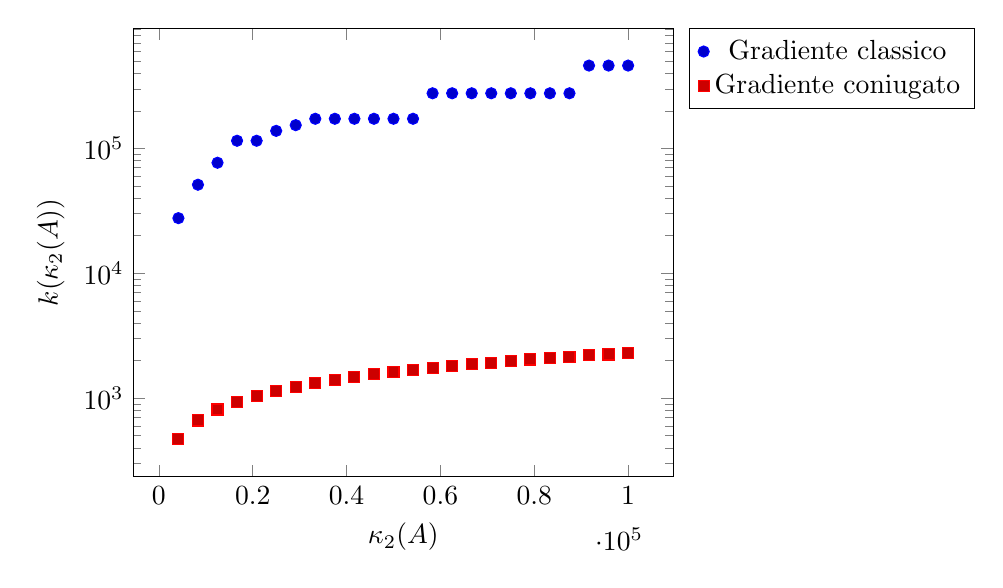
\begin{tikzpicture}
				\begin{axis}[xlabel = \(\kappa_2 (A)\), ylabel = \(k (\kappa_2 (A))\), only marks, domain = 1:100000, ymode = log, legend entries = {{Gradiente classico}, {Gradiente coniugato}}, legend pos = outer north east]
					\addplot {ceil(ln(10^(-6)) / ln((x - 1) / (x + 1)))};
					\addplot {ceil(ln(10^(-6) / 2) / ln((sqrt(x) - 1) / (sqrt(x) + 1)))};
				\end{axis}
			\end{tikzpicture}
			
			\caption{Confronto tra metodo del gradiente classico e metodo del gradiente coniugato relativamente al numero di iterazioni necessarie per ottenere un errore inferiore a \(10^{-6}\) al variare del condizionamento di \(A\).}\label{fig:confronto-grad}
		\end{figure}
	\end{osservazione}